\documentclass[11pt]{beamer}

%% Fonts
\usepackage[adobefonts]{ctex}

\usepackage{multicol}
%\usepackage{mathabx}
%\usepackage[scaled]{helvet}
%\usepackage{lmodern}
%\usepackage{eulervm}
%\usefonttheme[onlymath]{serif}
%\usefonttheme{professionalfonts}
%\usefonttheme{structurebold}
%\hypersetup{backref}
\usepackage{setspace}
\usepackage{bm}
\usepackage{pgf}

\spacing{1.5}

%% Color & Theme
\definecolor{SUblue}{RGB}{0,0,180}
\usecolortheme[RGB={0,0,180}]{structure}
\usetheme{Boadilla}
\setbeamertemplate{navigation symbols}{}
% \setbeamertemplate{itemize items}[circle]
% \setbeamertemplate{enumerate items}[circle]
\setbeamerfont{title}{size=\Huge}
\setbeamerfont{frametitle}{size=\Large}
% \setbeamerfont{framesubtitle}{size=\large,shape =$\color{violet}{\looparrowdownright}~$}
\setbeamercolor{title}{fg=white, bg= SUblue!75!green}
\setbeamercolor{framesubtitle}{fg=violet}
%\setlength{\leftmargini}{40pt}


\title[复杂模型应对复杂数据]{复杂模型应对复杂数据}

\author[李丰]{\large{李~~丰}}
\institute[中央财经大学]{\large{中央财经大学·统计与数学学院}}
\date{\texttt{feng.li@cufe.edu.cn}}


%%%%%%%%%%%%%%%%%%%%%%%%%%%%%%%%%%%%%%%%%%%%%%%%%%%%%%%%%%%%%%%%%%%%%%%%%%%%%%%
\begin{document}


%% Title page
\begin{frame}[plain]
  \titlepage
  \tiny{修订于\today}
\end{frame}


\begin{frame}
  \frametitle{李丰}

  \begin{itemize}

  \item  中央财经大学~~统计与数学学院~~副院长~~硕士生导师

  \item 教育背景

    \begin{tabular}{ l  p{0.75\textwidth} l}
      2008 --- 2013 &\textbf{统计学~博士}~~瑞典斯德哥尔摩大学统计学系\\
      % & 论文题目:\emph{贝叶斯条件密度估计方法}。\\
      % & 导师: Mattias Villani教授\\
      % & 答辩对手:Sylvia Frühwirth-Schnatter 教授。\\

      2007 --- 2008 & \textbf{统计学~硕士}~~ 瑞典达拉那大学统计学系\\

      2003 --- 2007 & \textbf{统计学~本科}~~ 中国人民大学统计学院\\
    \end{tabular}

  \item 研究兴趣

    \begin{itemize}
    \item 大数据与复杂模型
    \item 贝叶斯推断与统计计算
    \item 计量经济与预测方法
    \item 多元模型

    \end{itemize}

  \end{itemize}


\end{frame}



%% Outline page
% \section*{Outlines}
% \begin{frame}
%   \frametitle{Outlines}
%   \tableofcontents
% \end{frame}
%%%%%%%%%%%%%%%%%%%%%%%%%%%%%%%%%%%%%%%%%%%%%%%%%%%%%%%%%%%%%%%%%%%%%%%%%%%%%%%


\begin{frame}
  \frametitle{你是否曾经想过?}

  \begin{itemize}
  \item 为什么天气预报有些时候不准?
  \item 电子邮件的垃圾过滤器如何区分正常邮件和垃圾邮件?
  \item 我们是否可以预测下一次金融危机?
  \item 我们通过停车场自动收费系统时,它如何自动扫描到我们的车牌?
  \end{itemize}
  \vspace{1cm}所有这些都涉及到一个问题——即通过\textbf{模型}来描述\textbf{数据}之间的关系并
  为人们的决策提供依据。
\end{frame}

% \section{The trend of data we see}

\begin{frame}
  \frametitle{简单模型示例:父亲的身高与儿子的身高}
  \centering 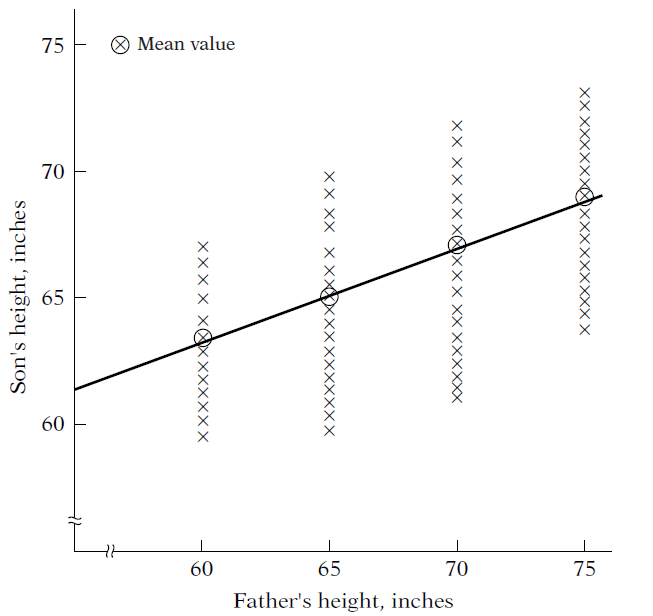
\includegraphics[height=0.8\textheight]{father_son}\\
  \tiny{Gujarati, D. N. (2003). Basic Econometrics. 4th.}
\end{frame}

\begin{frame}
  \frametitle{简单模型示例:家庭收入与支出}
  \centering 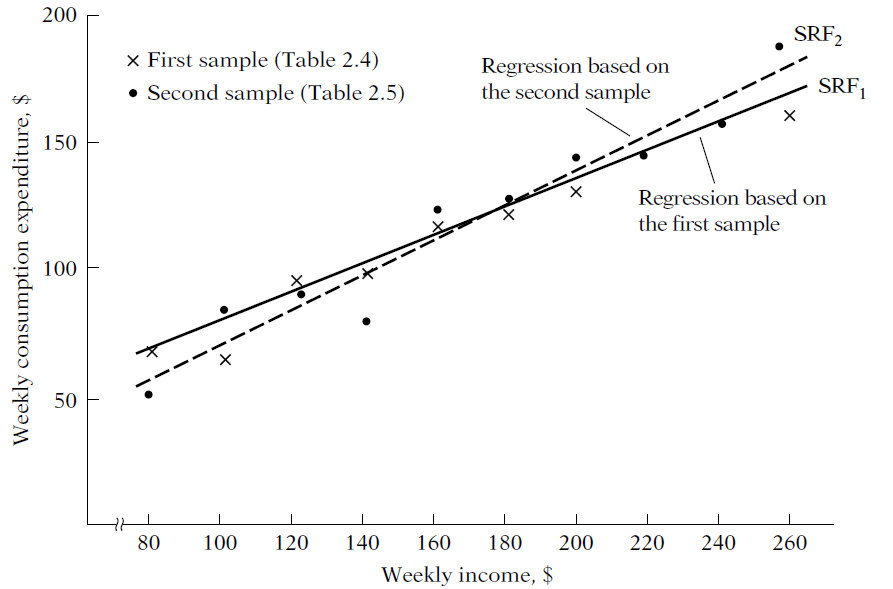
\includegraphics[height=0.8\textheight]{family_income_sample_line}\\

  \tiny{Gujarati, D. N. (2003). Basic Econometrics. 4th.}
\end{frame}

\begin{frame}
  \frametitle{简单模型的特点}
  \begin{itemize}
  \item 模型使用的\textbf{数学工具}、\textbf{计算方法}、\textbf{描述的关系} 相对简单。
  \item 在很多常见场景里非常有用。
  \item 而且计算方便。
  \item 模型描述的关系容易通过图形展示。
  \item 在很多常用的计算机软件里集成了计算工具。
  \end{itemize}

\end{frame}

\begin{frame}
  \frametitle{复杂数据示例:股票收益}
    \centering 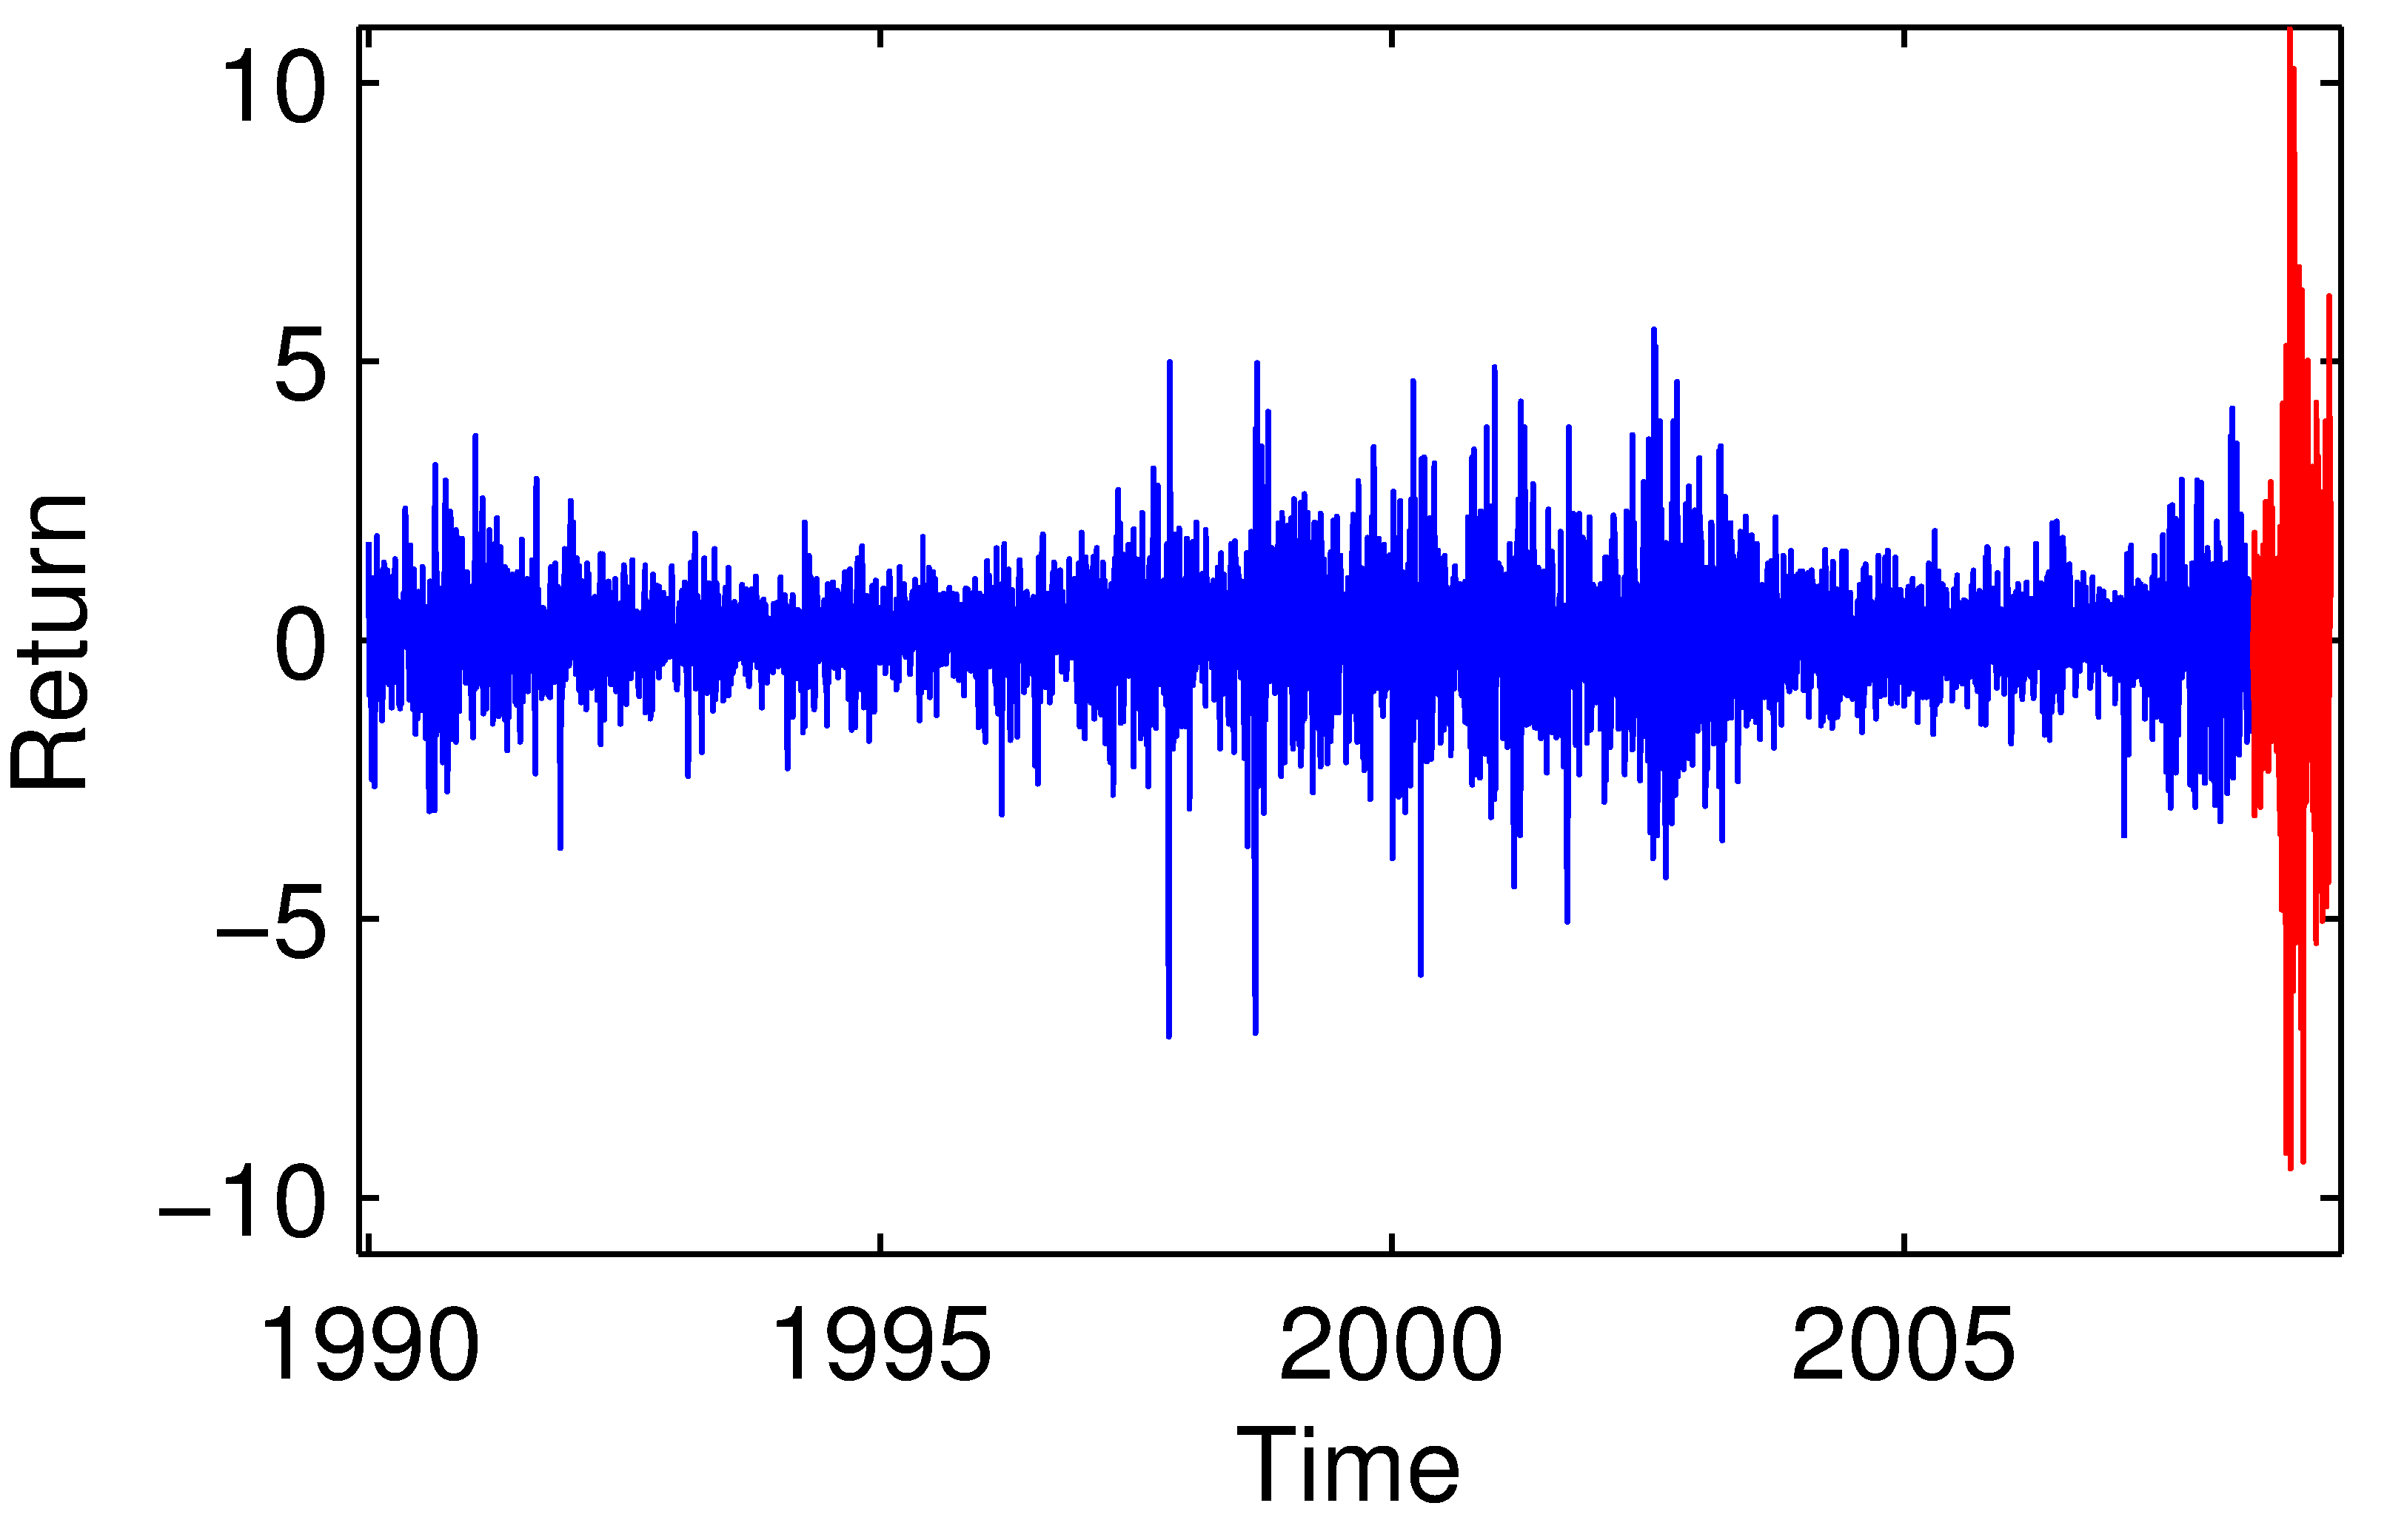
\includegraphics[height=0.8\textheight]{return}
\end{frame}




\begin{frame}
  \frametitle{股票收益:历史收益 vs 现收益}
    \centering 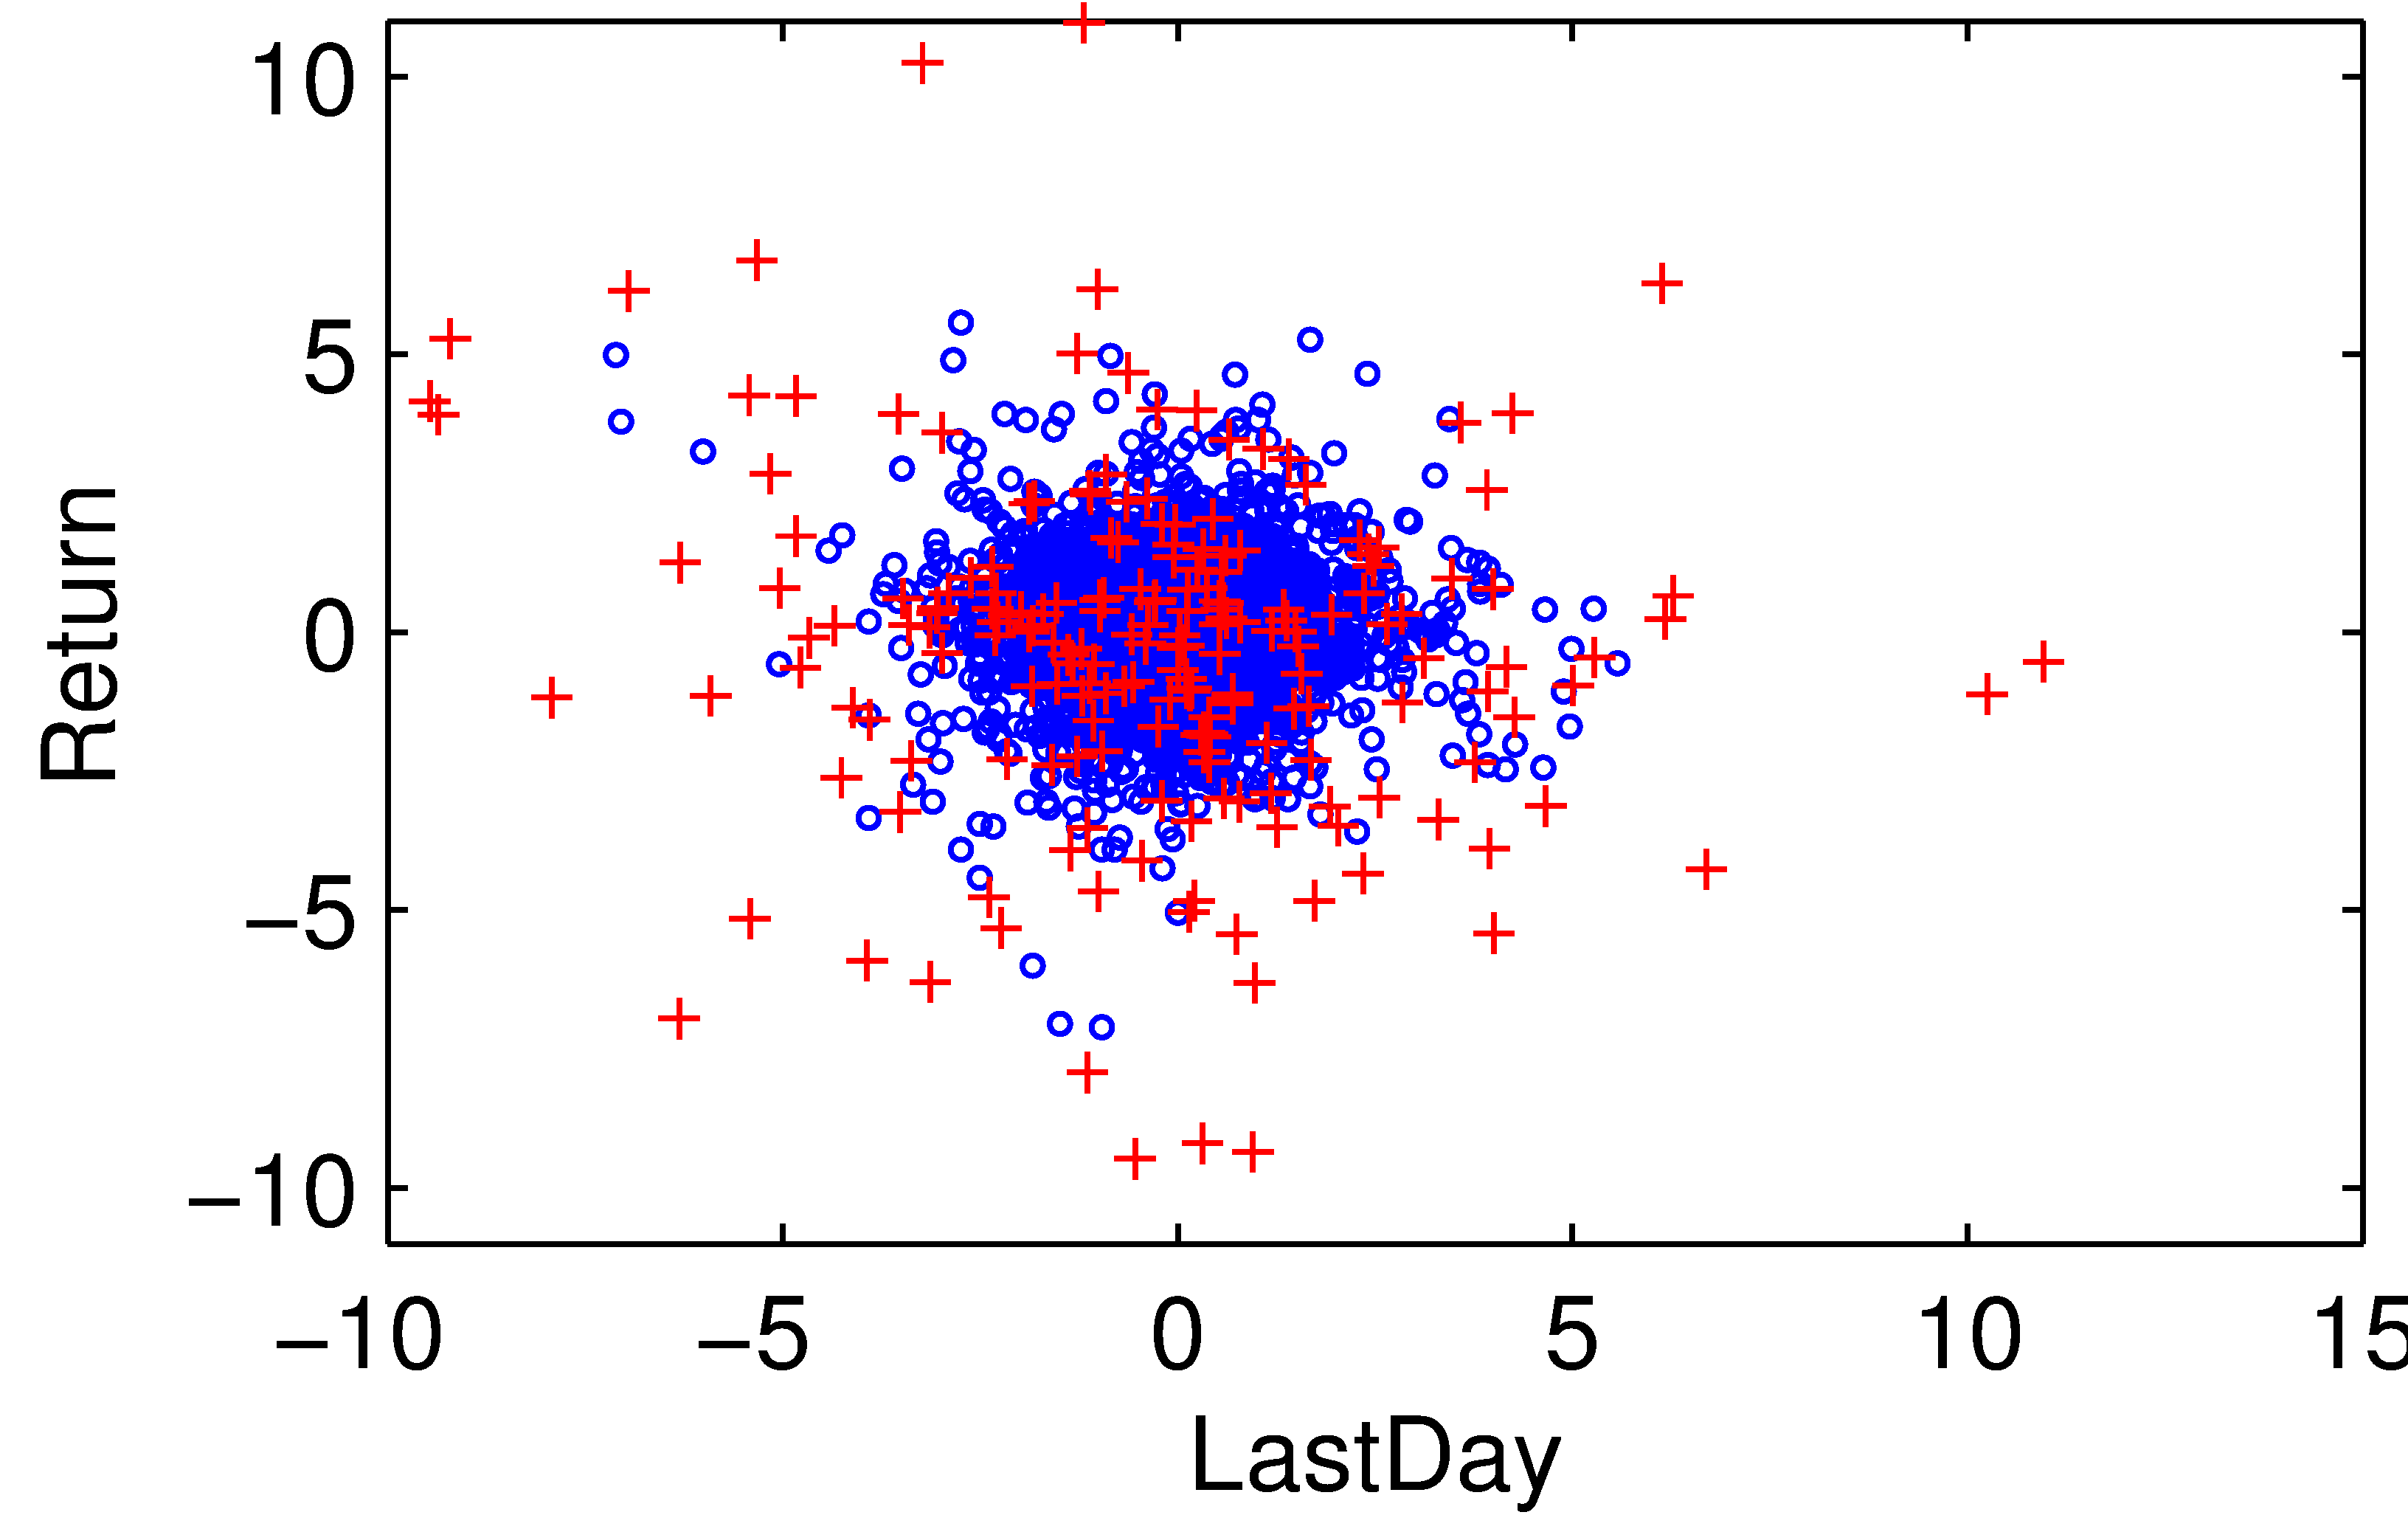
\includegraphics[height=0.8\textheight]{returnlastday}
\end{frame}

\begin{frame}
  \frametitle{股票收益数据:历史收益\textbf{波动}vs现收益}
  \centering 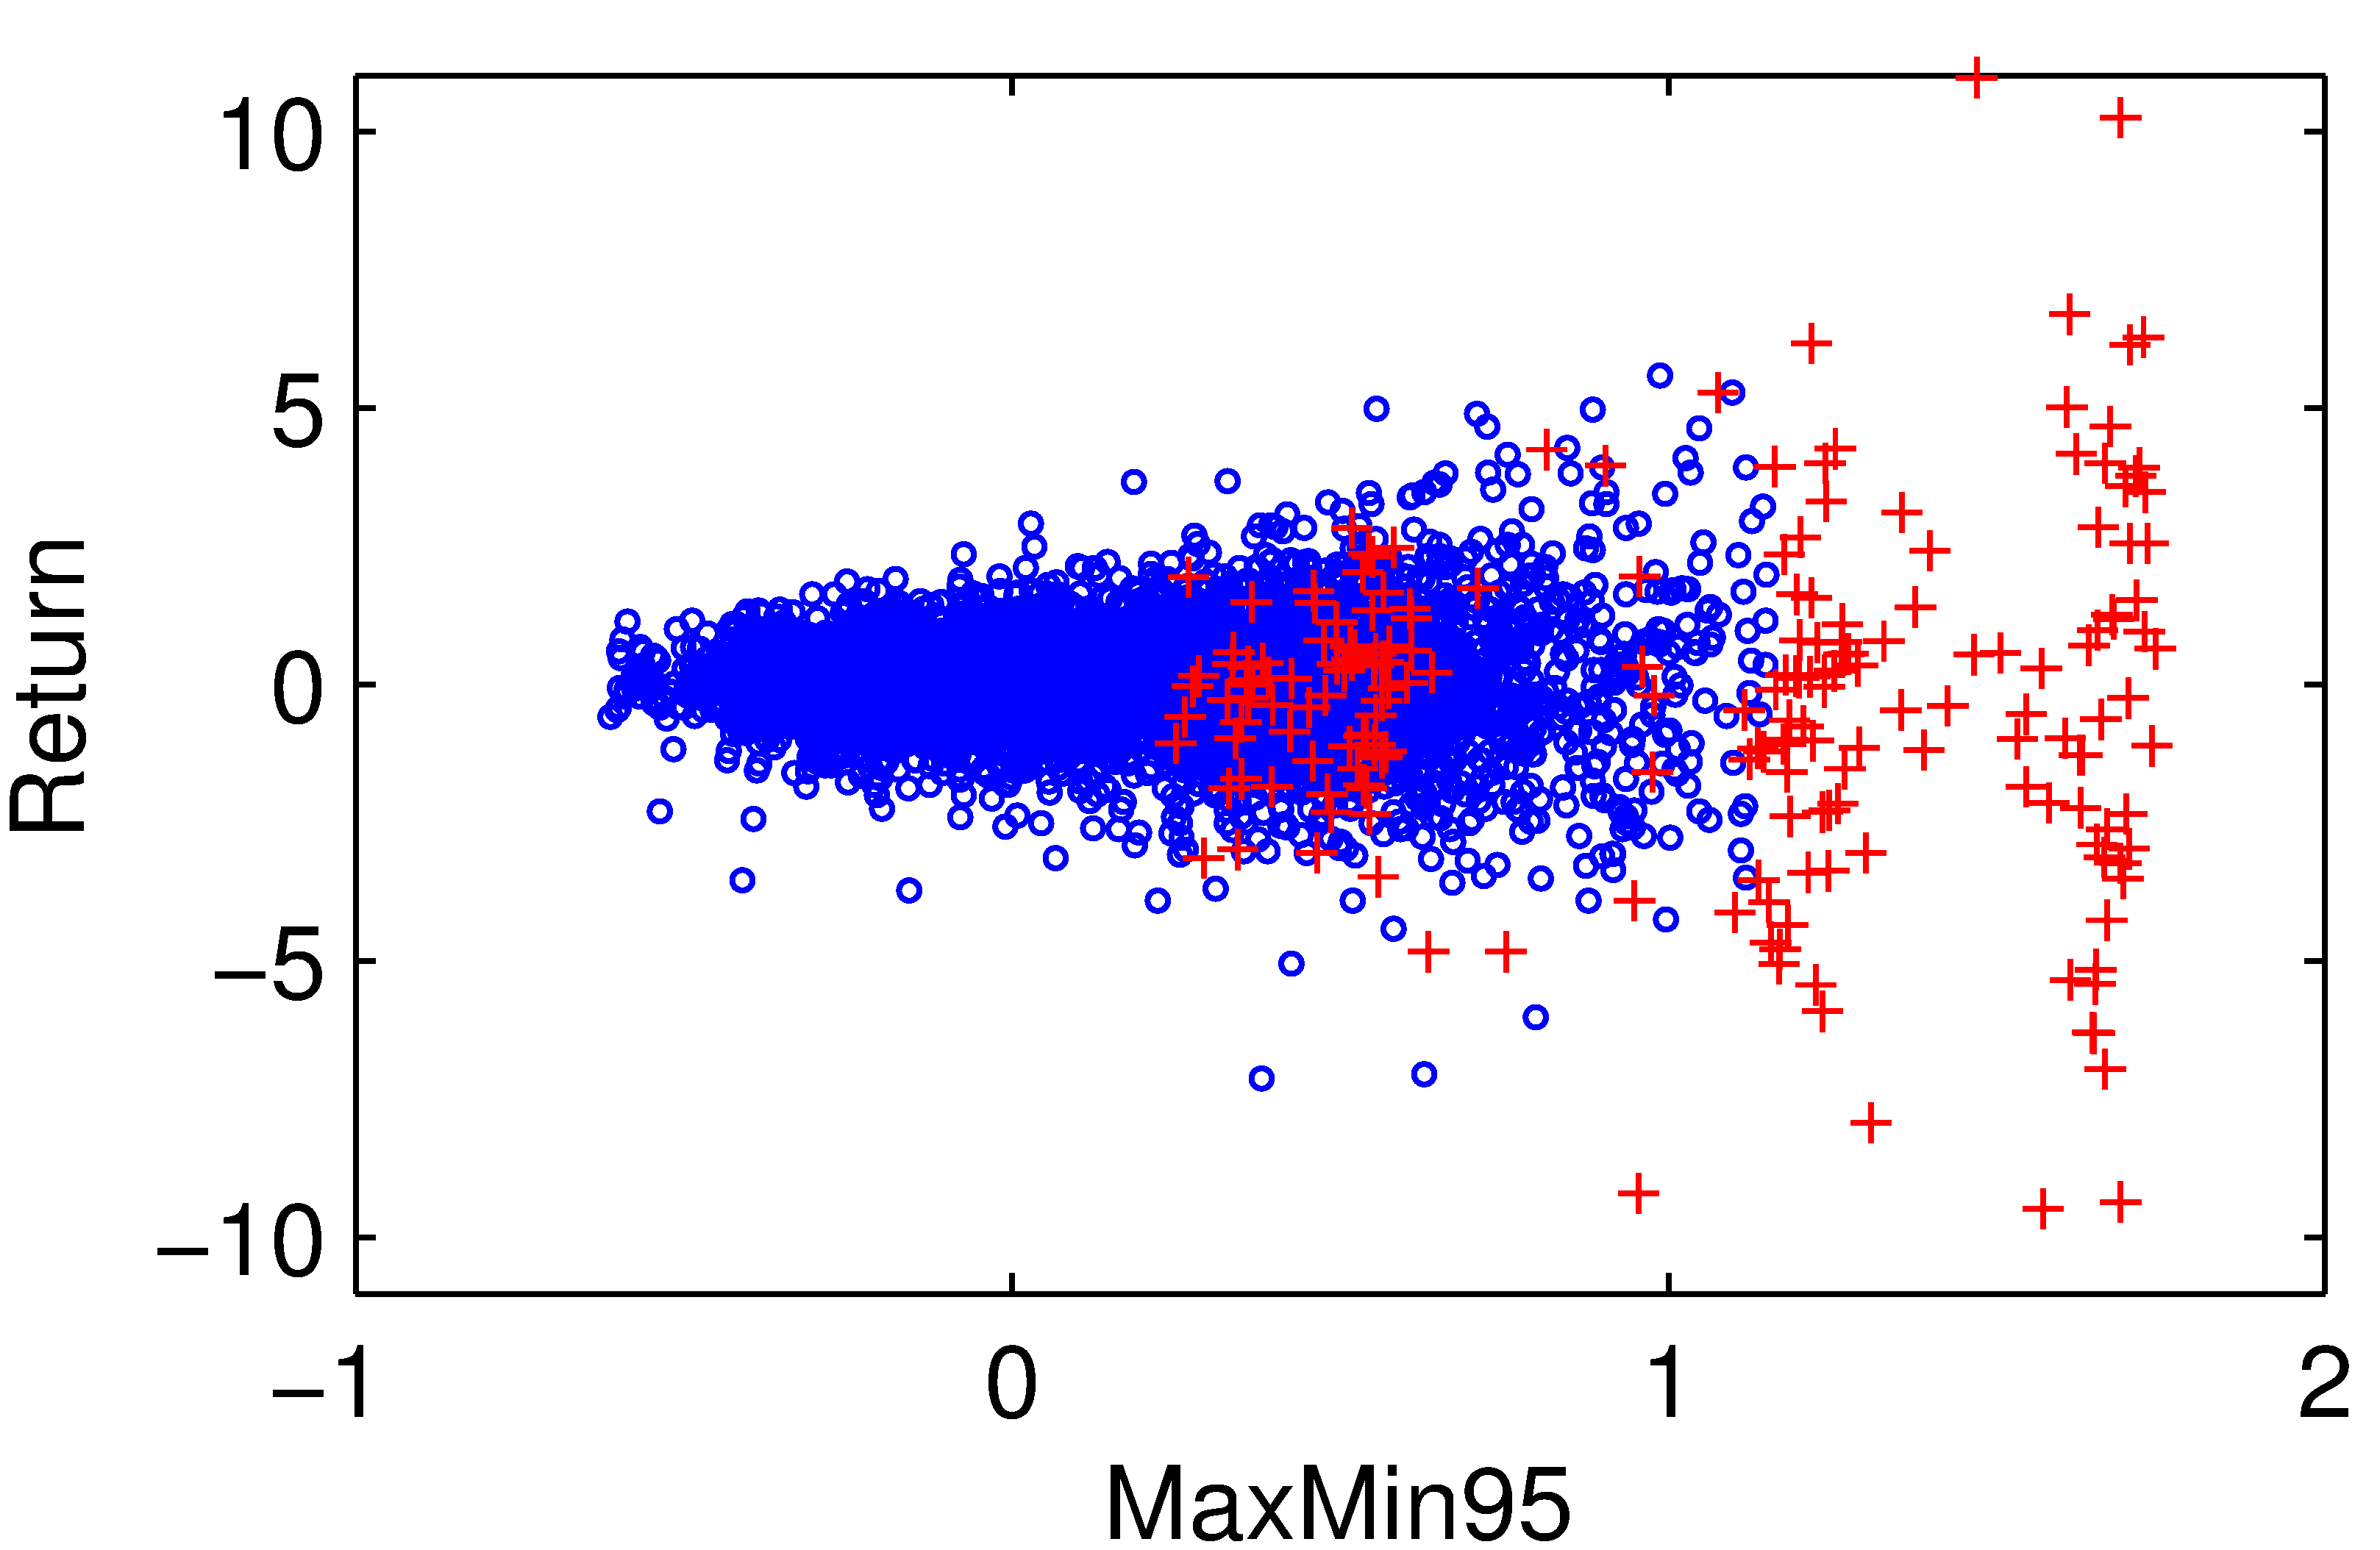
\includegraphics[height=0.8\textheight]{returnminmax}
\end{frame}


\begin{frame}
  \frametitle{复杂数据特征}
  \begin{itemize}
  \item 股票数据看起来并不是 \textbf{正态的} (考虑均值和方差)
  \item 如何用统计模型正确描述这种特殊的数据呢?

    \begin{itemize}
    \item 用 \textbf{均值}和\textbf{方差} (\emph{或者标准差}) 来描述正态性。
    \item 用 \textbf{偏态}和\textbf{峰态} (\emph{或者自由度}) 来描述非正态特征。
    \end{itemize}

  \end{itemize}
\end{frame}

\begin{frame}
  \frametitle{正态和非正态}
  \begin{figure}
    \centering
     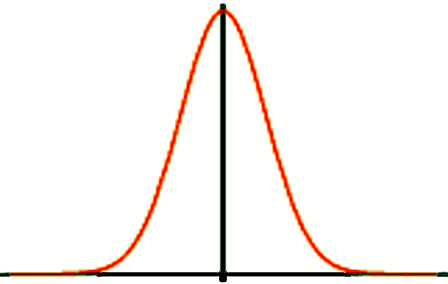
\includegraphics[height=0.35\textheight]{normal}\\
     Normal\\
     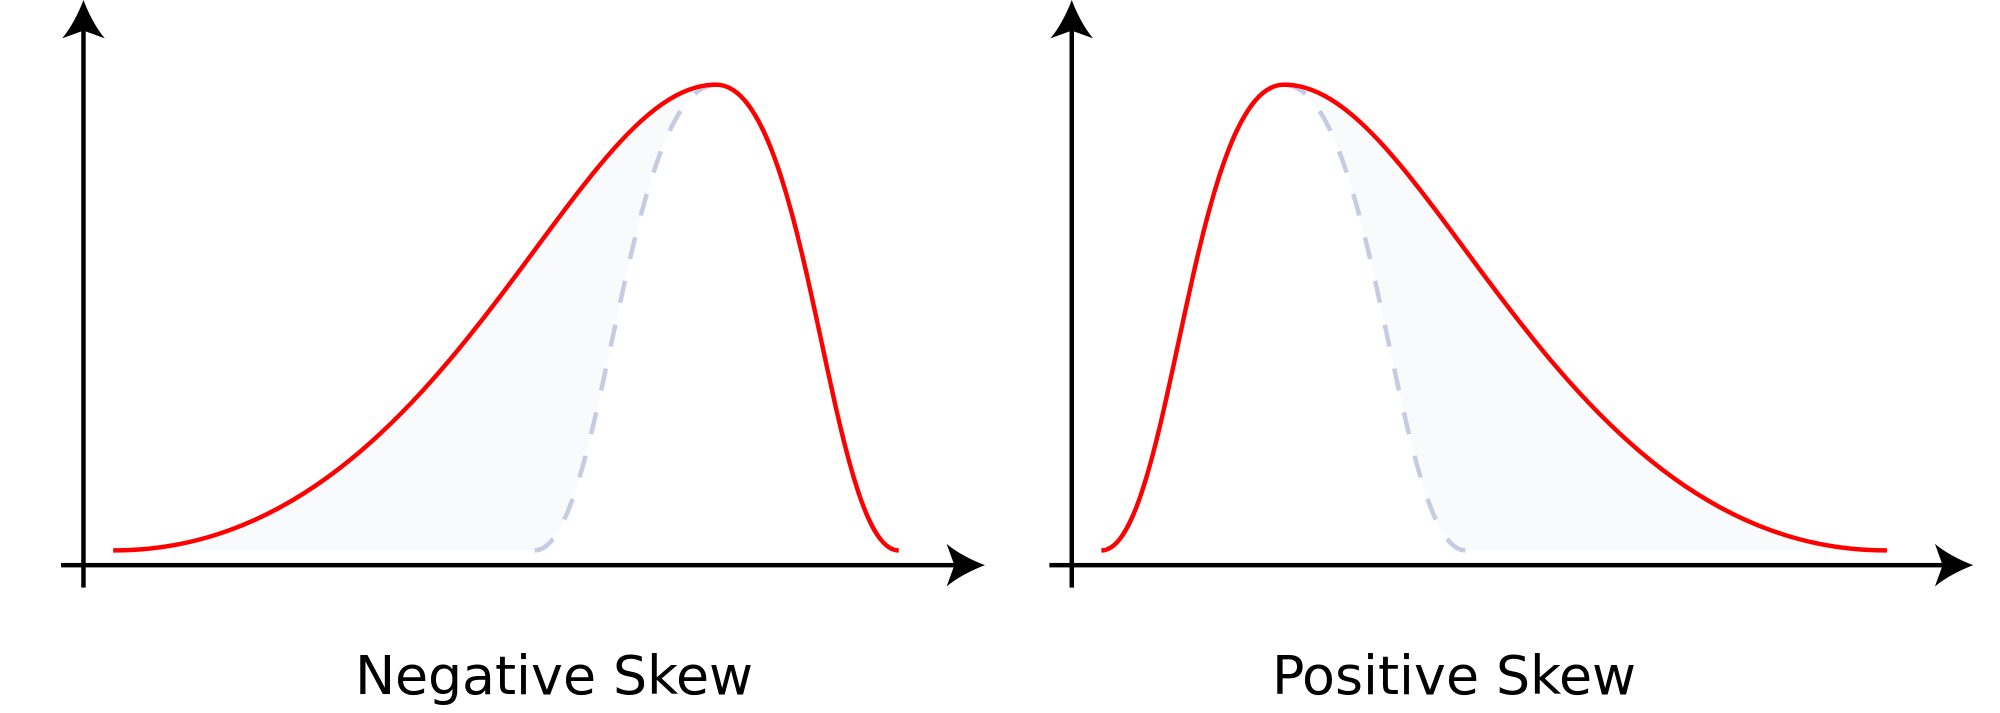
\includegraphics[height=0.35\textheight]{skew}
  \end{figure}
\end{frame}


\begin{frame}
  \frametitle{复杂模型:金融危机预警}
  \begin{figure}
    \centering
    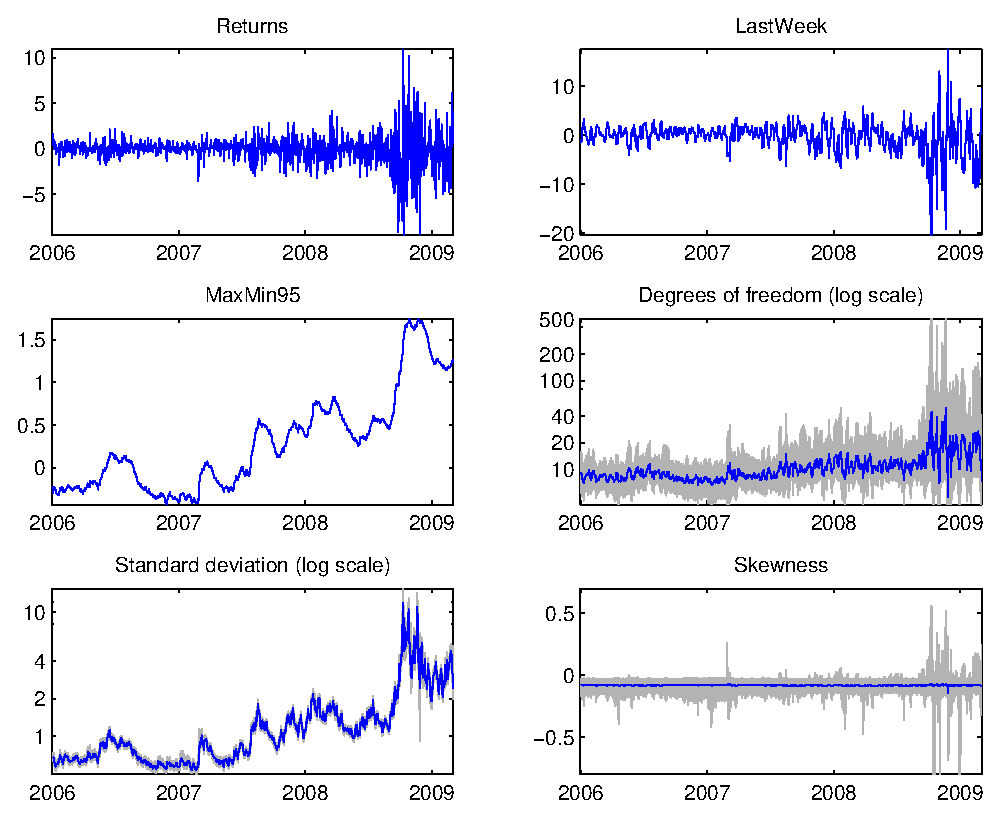
\includegraphics[height=0.85\textheight]{MomentPlotSP5002}
  \end{figure}
\end{frame}


\begin{frame}
  \frametitle{为什么金融危机还是发生了? }
\begin{itemize}
\item  因为用了错误的模型!
\item  如果用错模型会怎么样?
  \begin{itemize}
  \item 模型将不会被正确识别。
  \item 所有基于该模型的结论都有可能是错误的。
  \end{itemize}

\item 但是为什么人们仍然在使用错误的模型?

  \begin{itemize}
  \item 错误的模型往往简单易用。
  \item 使用者并不知道模型本来就是错的。
  \end{itemize}

\end{itemize}
\end{frame}



\begin{frame}
  \frametitle{复杂数据:多元股票数据}
  \begin{figure}
    \centering
    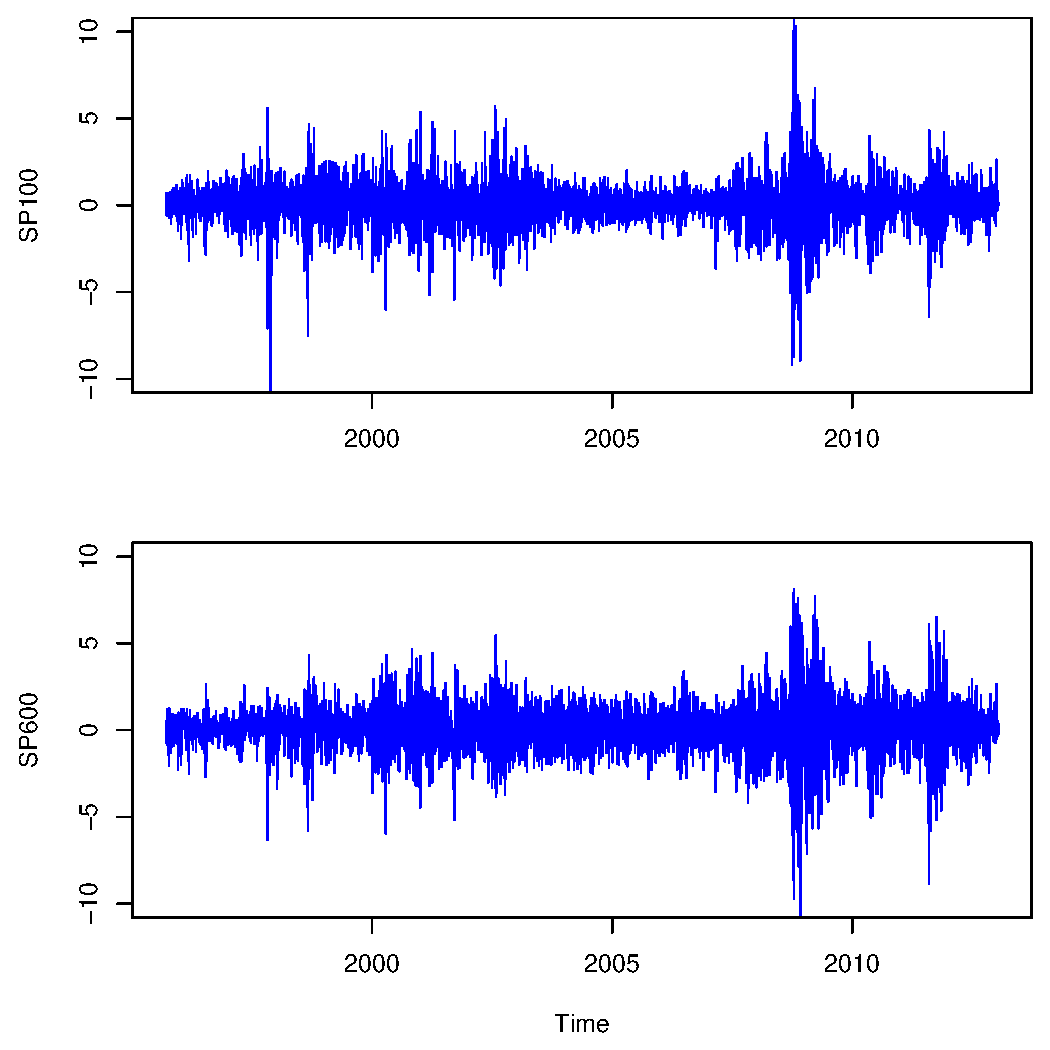
\includegraphics[height=0.9\textheight]{SP100-SP600}
  \end{figure}
\end{frame}

\begin{frame}
  \frametitle{复杂数据:多元股票数据}

  \begin{itemize}

  \item 我们不仅仅关注个股的股票收益,我们更关心多只股票(大盘)的联合波动

  \item 如果某只股票跌停,其他股票也跌停的概率有多大?(\textbf{尾部相依性})

  \item 哪些因素影响到这些概率?
  \end{itemize}

\end{frame}

\begin{frame}
  \frametitle{股票的尾部相依性}
  \begin{figure}
    \centering
    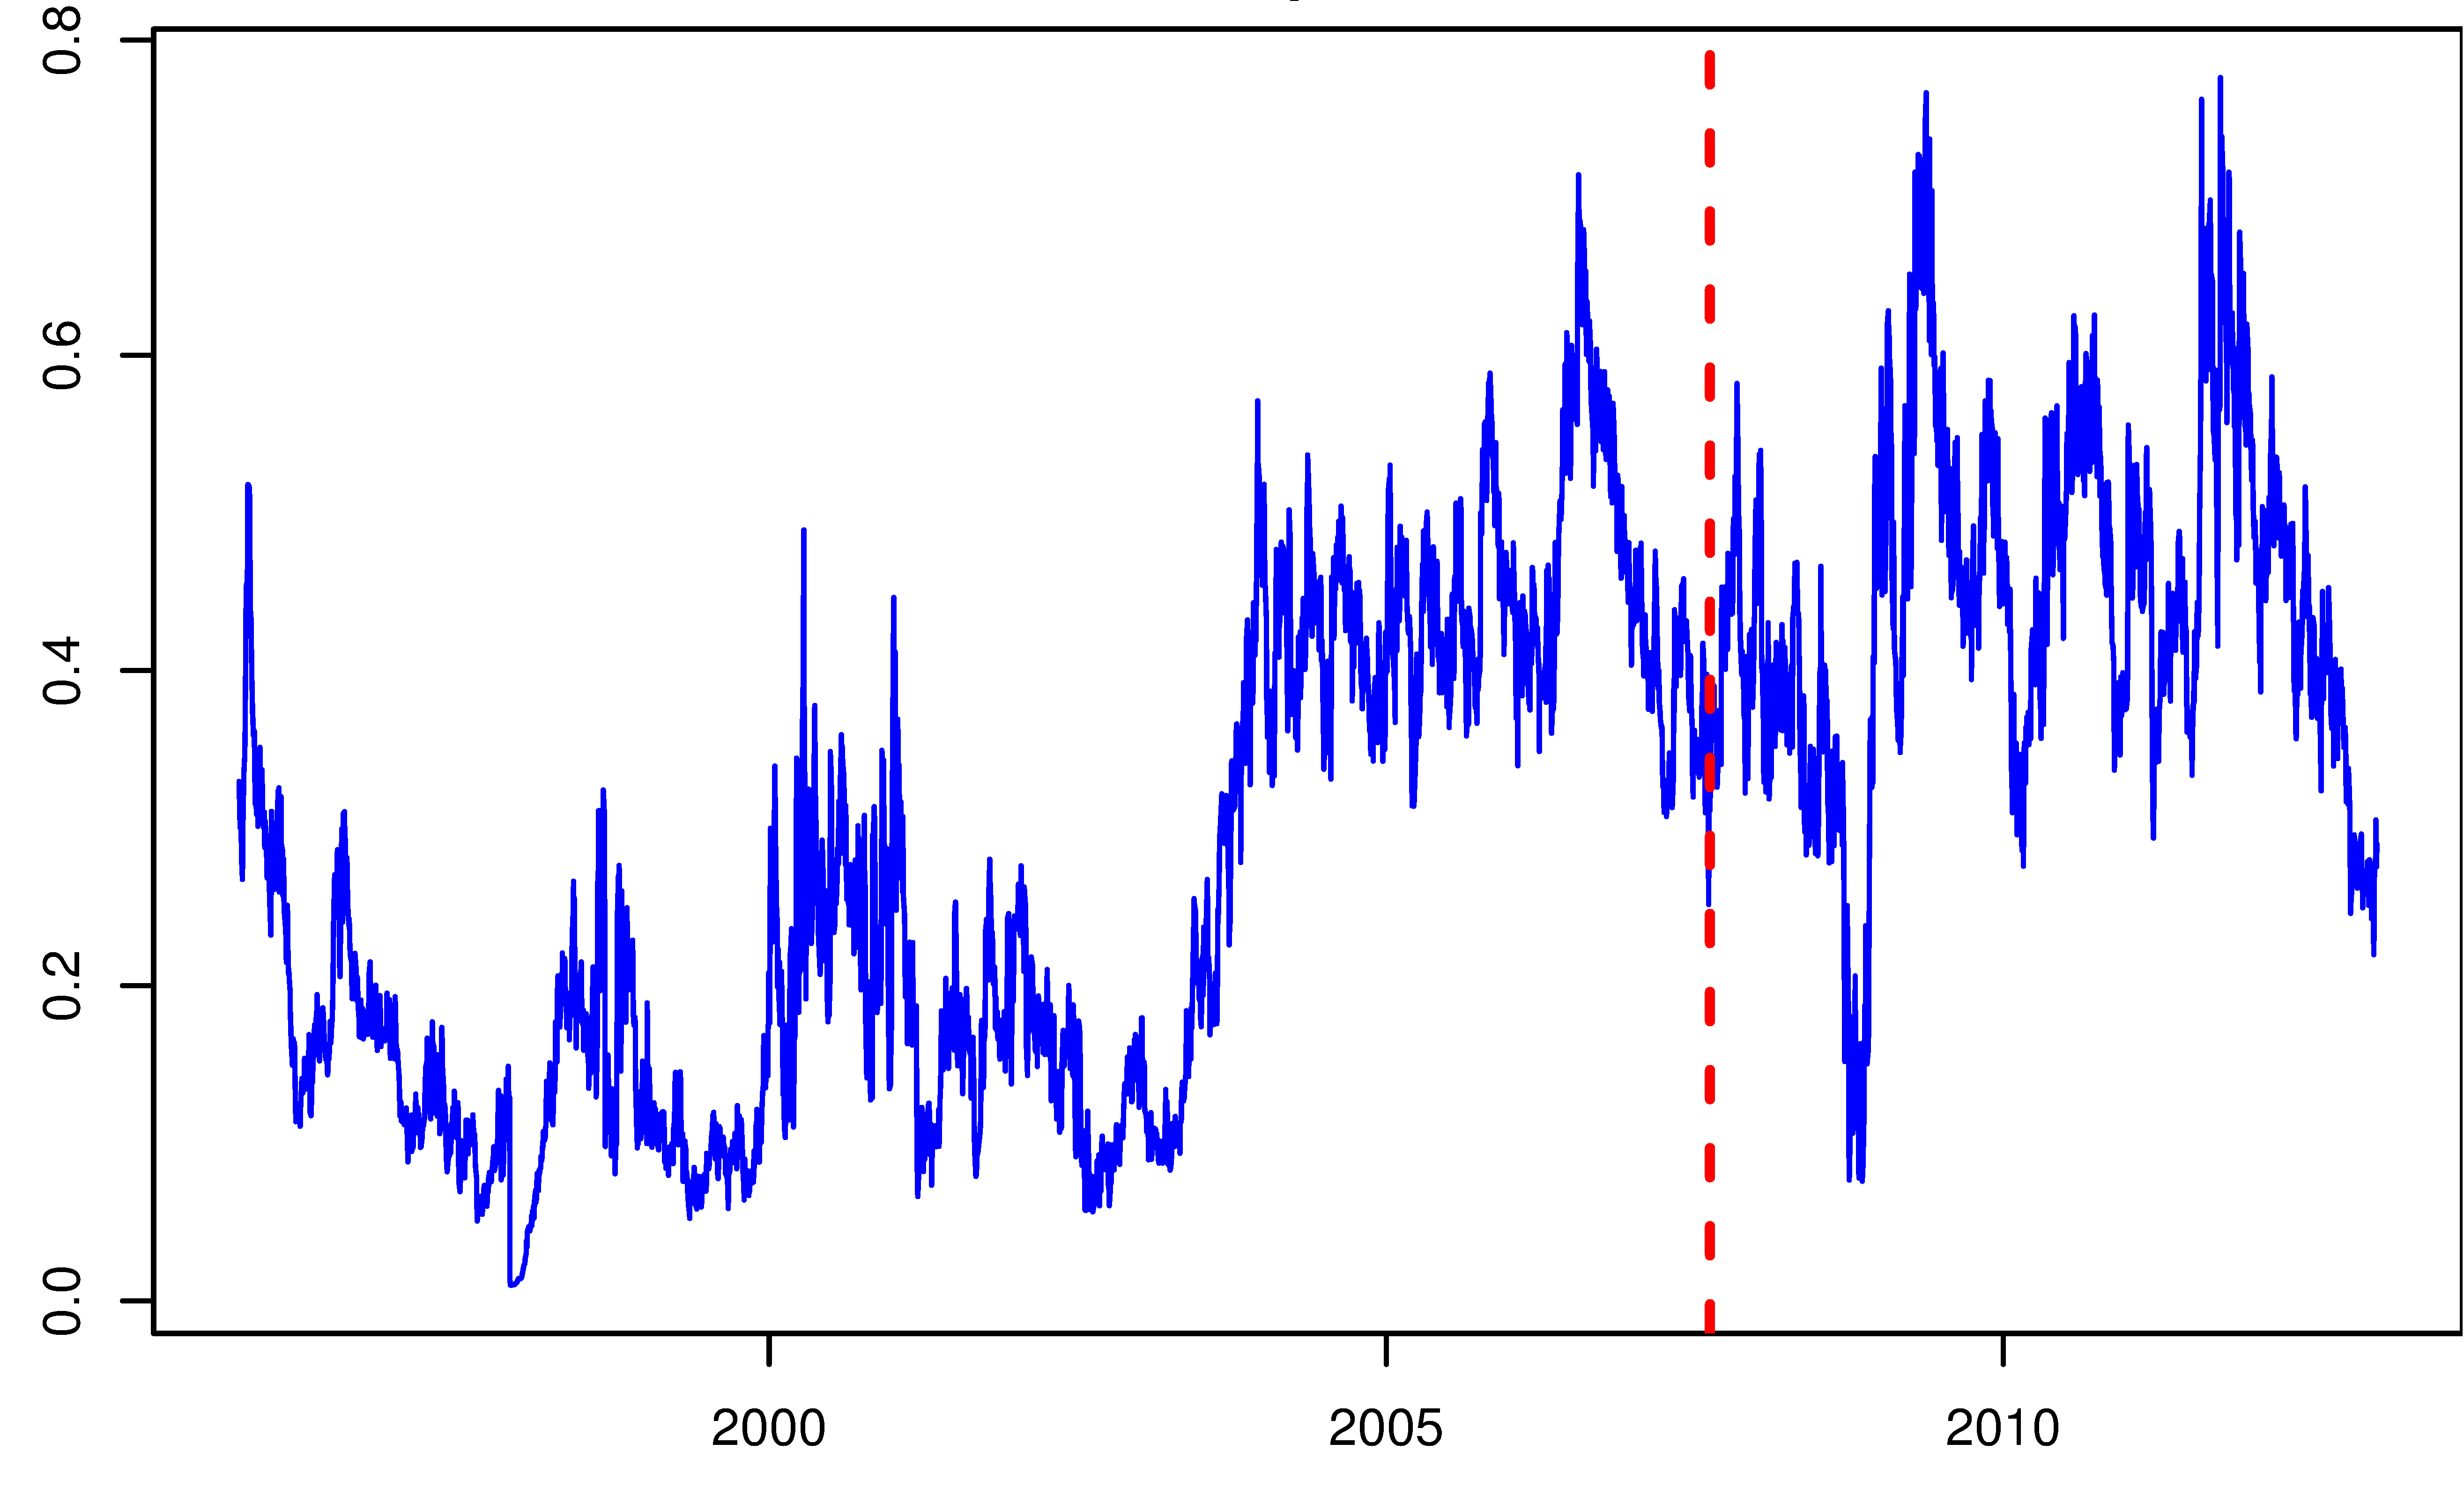
\includegraphics[height=0.75\textheight]{tail-dep}
  \end{figure}
\end{frame}



\begin{frame}
  \frametitle{复杂数据:股票收益与新闻文本}
  \begin{figure}
    \centering
    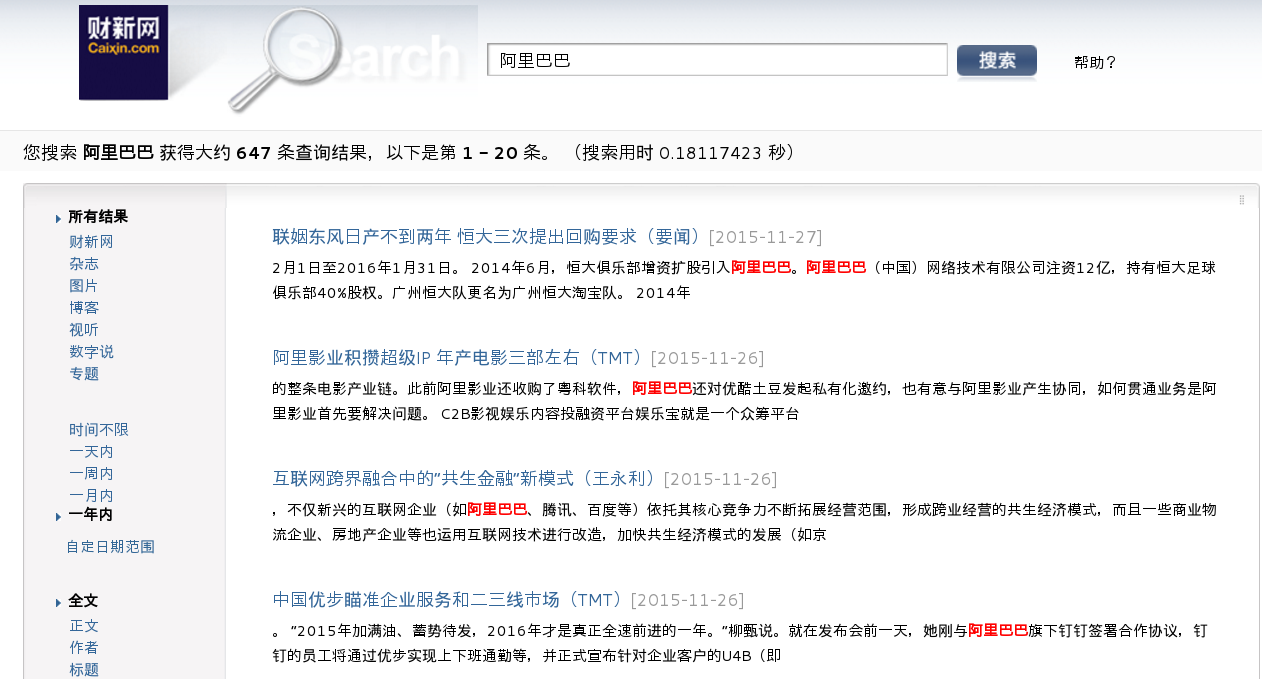
\includegraphics[height=0.7\textheight]{plot/Caixin.png}
  \end{figure}

\end{frame}


\begin{frame}
  \frametitle{新闻主题的演进与股票波动}
  \begin{figure}
    \centering
    
\includegraphics[height=0.28\textheight]{plot/Sep-Oct-wordcloud}    
\includegraphics[height=0.28\textheight]{plot/Nov-wordcloud}
    
\includegraphics[height=0.28\textheight]{plot/Dec-wordcloud}\\
    
\includegraphics[height=0.28\textheight]{plot/Jan-wordcloud}    
\includegraphics[height=0.28\textheight]{plot/Feb-wordcloud}
    
\includegraphics[height=0.3\textheight]{plot/Mar-Apr-wordcloud}\\
    
\includegraphics[height=0.3\textheight]{plot/May-wordcloud}    
\includegraphics[height=0.3\textheight]{plot/Jun-wordcloud}
    
\includegraphics[height=0.3\textheight]{plot/Jul-wordcloud}\\

  \end{figure}
\end{frame}

\begin{frame}
  % \frametitle{The stock market returns for two indices}
  \begin{figure}
    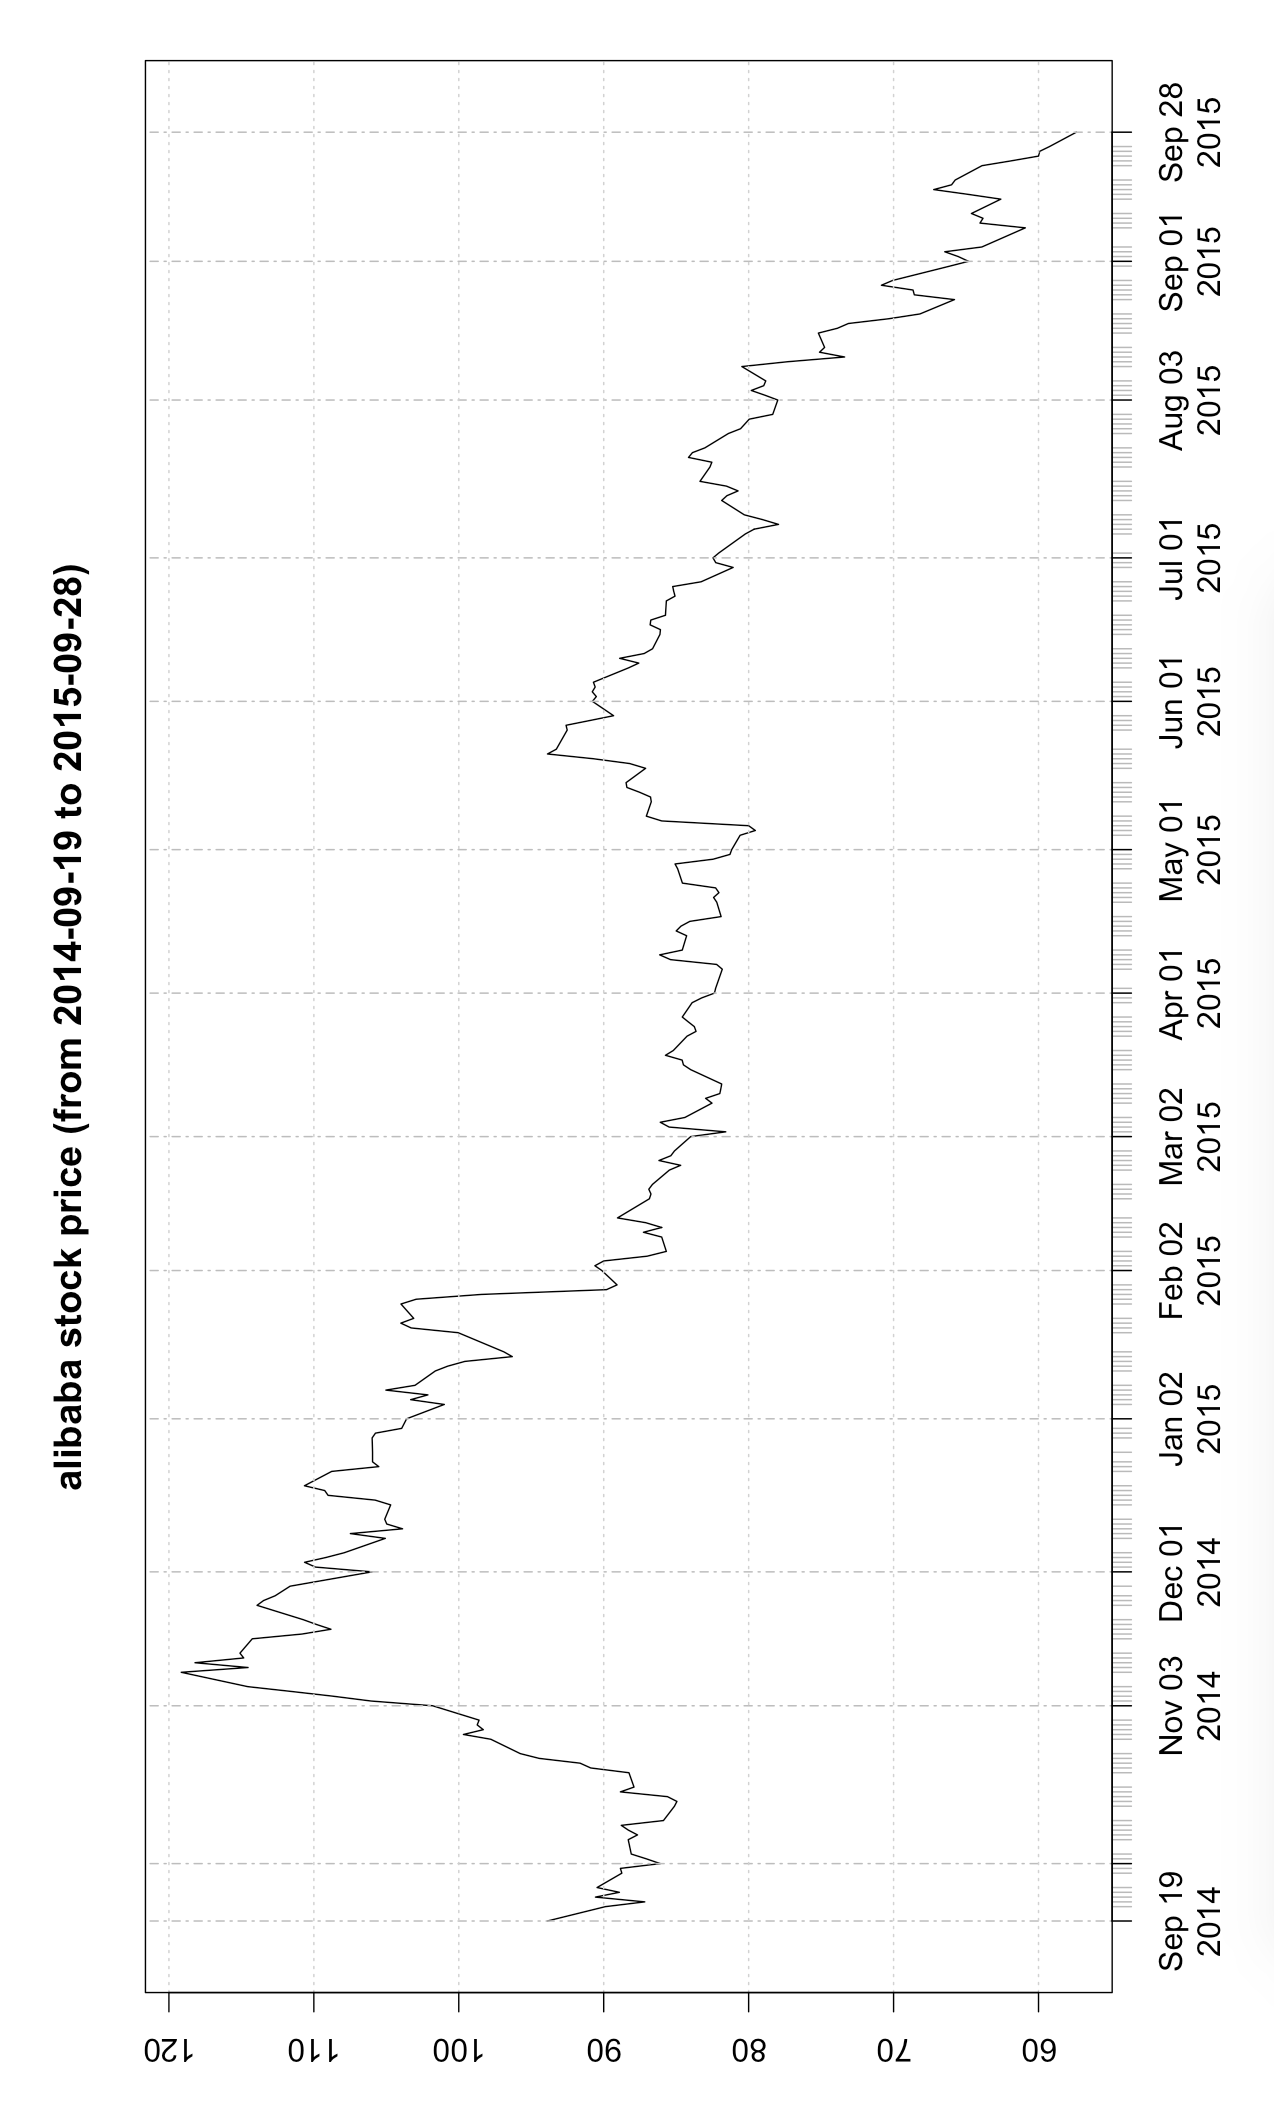
\includegraphics[width=0.45\textwidth]{plot/Alibaba-Stock-Price-R.png} 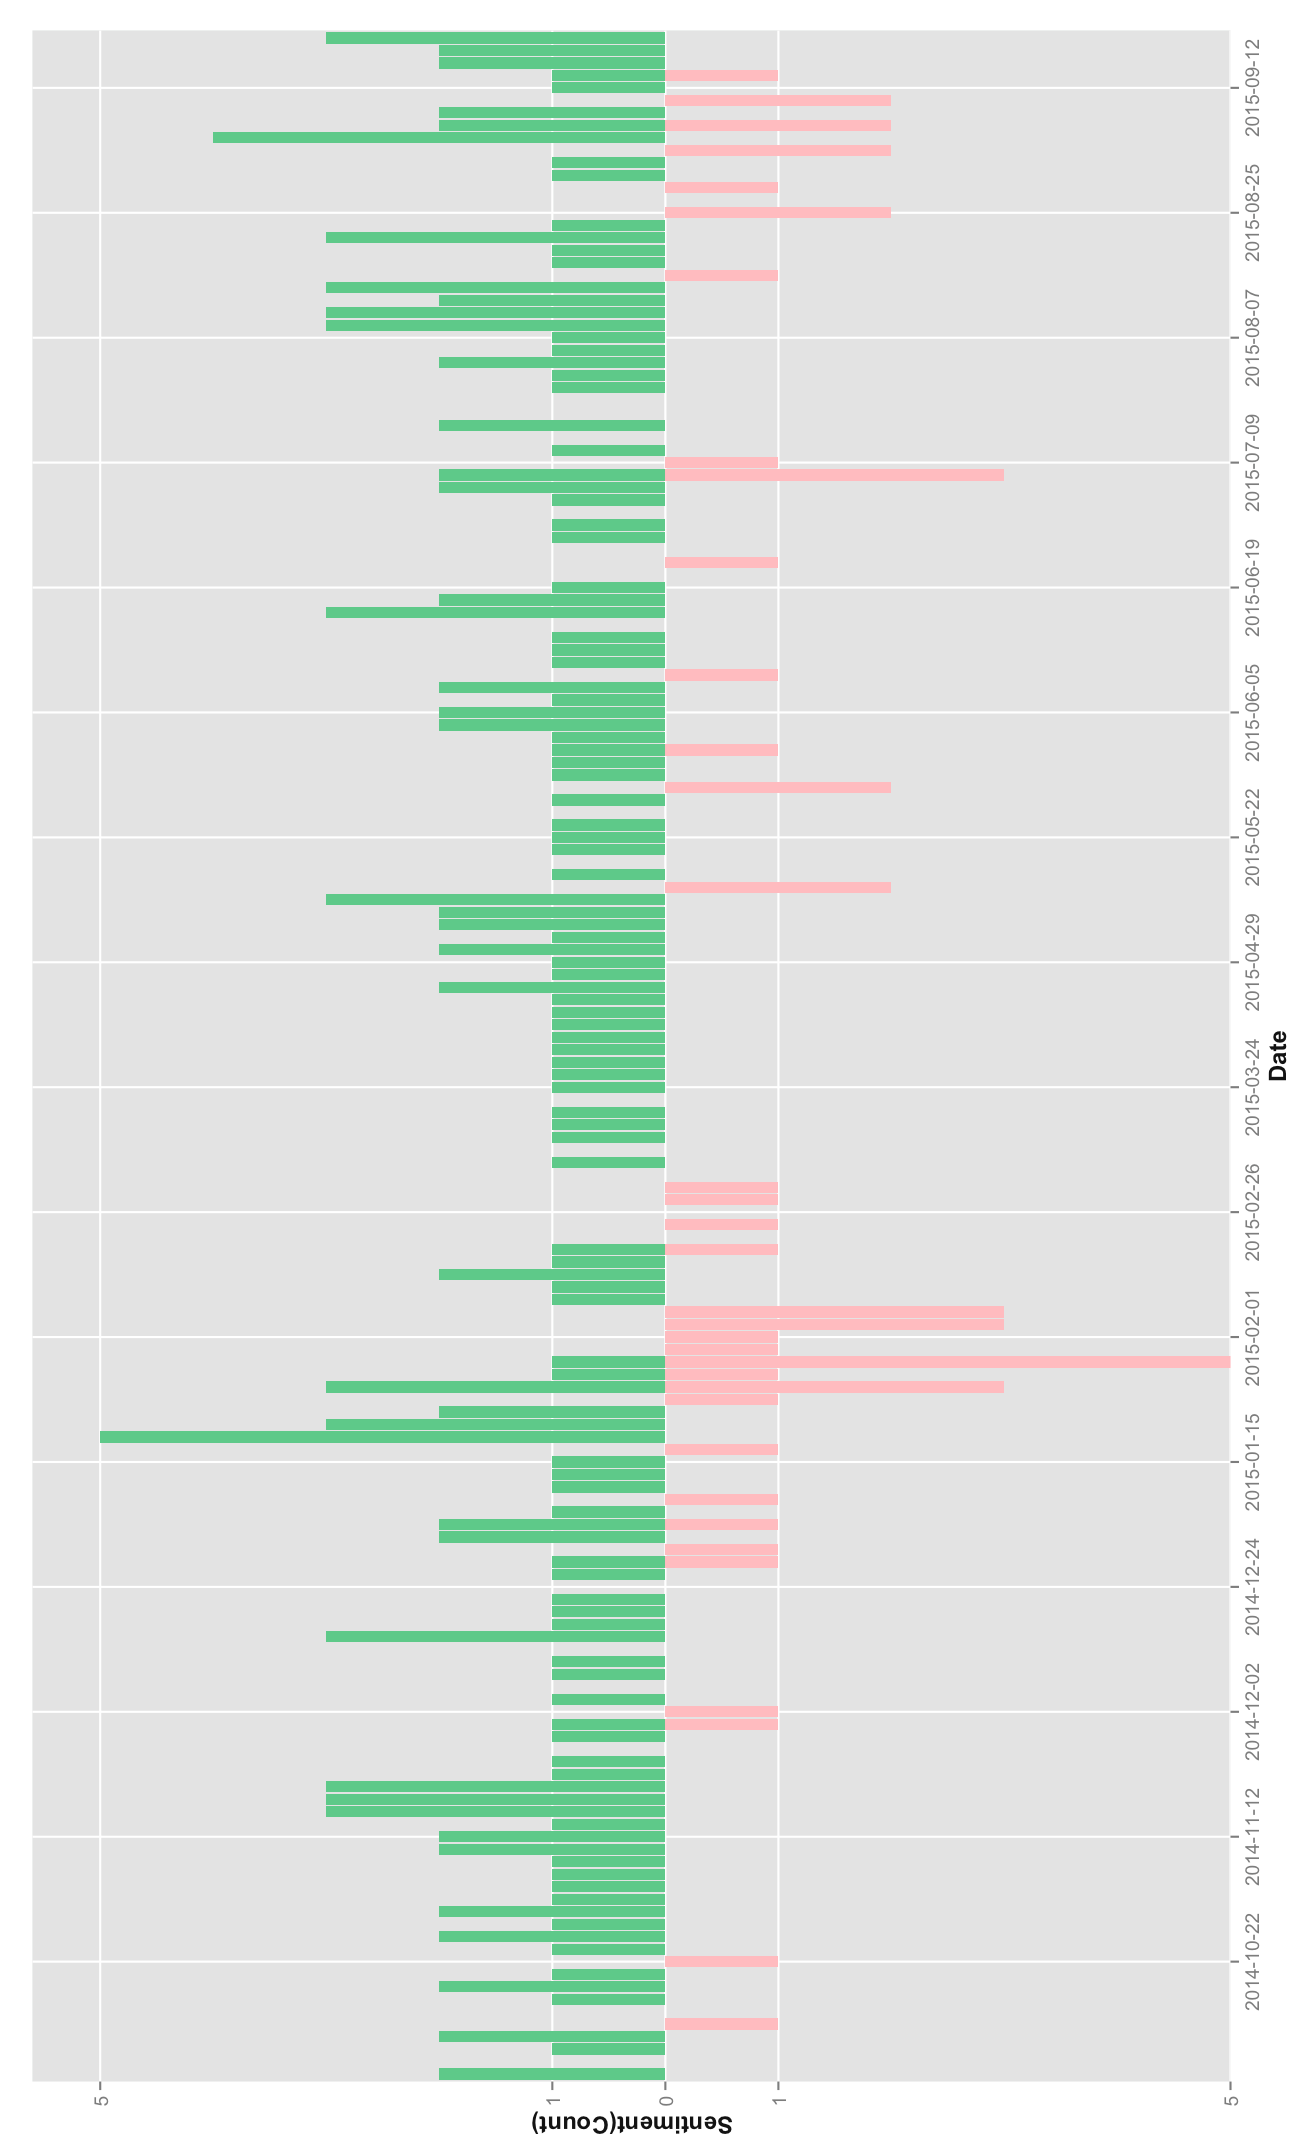
\includegraphics[width=0.45\textwidth]{plot/Sen-Date.png}
  \end{figure}
\end{frame}

\begin{frame}
  \frametitle{新闻情绪是如何影响股票波动的?}
  \begin{figure}
    \centering
    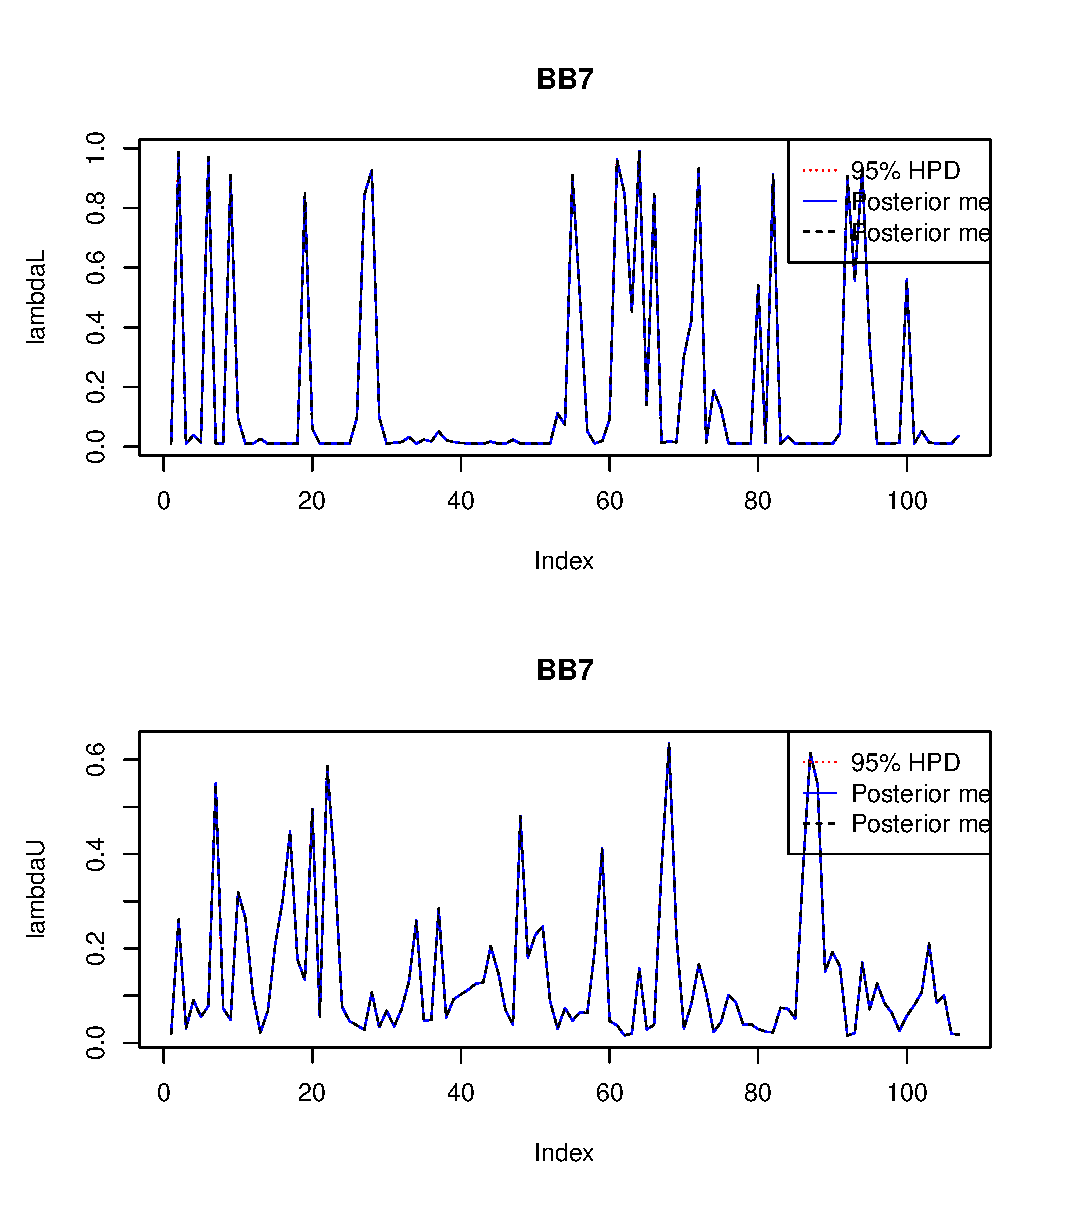
\includegraphics[height=0.9\textheight]{plot/lambdaLU}\\
    % \hspace{-1cm}
\includegraphics[height=0.41\textheight]{tau-post}
  \end{figure}
\end{frame}



\begin{frame}
  \frametitle{模型和数据的发展趋势}
  %\framesubtitle{The trend of statistical modeling}

  \begin{itemize}
  \item 上个世纪五十年代,线性模型被认为是非常先进的方法而现在是大学教科书的基础内容。
  \item 全世界90\%的数据在过去五年被创造。
    \begin{itemize}

    \item 据估计2012年全球所有存储数据为2.7ZB。
    \item 1克DNA中可以储存360EB的信息量。
    \item 在2009年,阿凡达3D版使用了多于1PB来储存。
    \item Google服务器的估计容量大约是5.625PB(截止2004年)。
    \item 国会图书馆 (美国)藏品数量的估计近似值大约是10PB(包括非书籍资料, 截止2005年)。
    \item 在2012年的8日, Facebook 共使用了约100PB。
    \item 全世界印刷材料的内容总量大约是300PB。
    \end{itemize}
  \end{itemize}
\end{frame}



\begin{frame}
  \frametitle{统计建模的一般过程}

  \begin{itemize}
  \item 数据采集:传统的报表式采集$\Rightarrow$ 大数据采集
  \item 模型估计:传统的单机软件傻瓜式操作$\Rightarrow$ 大数据分布式计算
  \item 模型评价
  \item 模型比较
  \item 模型预测
  \end{itemize}
\end{frame}


\begin{frame}
  \frametitle{简单模型 vs 海量数据}

    \centering 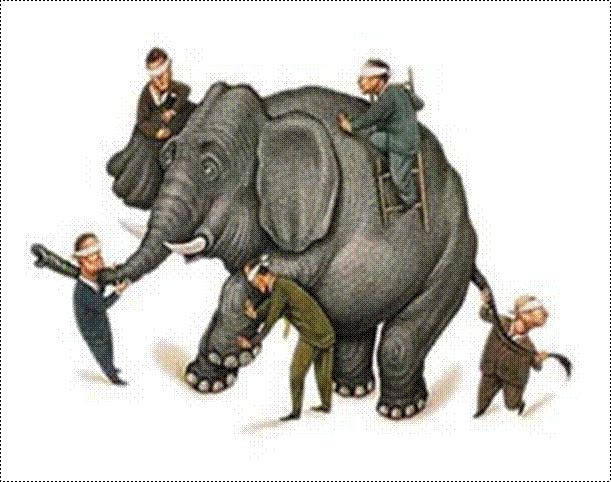
\includegraphics[height=0.75\textheight]{elephant}\\
    \tiny{John Godfrey Saxe (1816-1887)}
\end{frame}


\begin{frame}
  \frametitle{了解数据的本质需要复杂模型}

  \begin{itemize}
  \item 应对复杂数据,复杂模型是必需的。
  \item 复杂模型能够更加精细地捕捉数据的复杂特征。
  \item 但是估计复杂模型不是一件容易的事情。
    \begin{itemize}
    \item 现在的计算机还不够快。
    \item 对于传统的统计工作者而言,现代模型的计算机门槛高。
    \item 不幸的是错误的模型经常被使用。
    \end{itemize}
  \end{itemize}
\end{frame}


\begin{frame}
  \frametitle{但是要用对模型}

    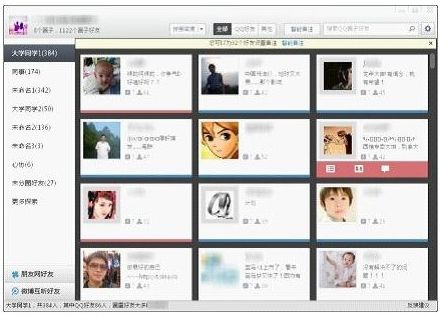
\includegraphics[width=0.8\textwidth]{QQRecommend}


\end{frame}


\begin{frame}[plain]
  \addtocounter{framenumber}{-1}
\begin{multicols}{2}
  
\includegraphics[width=0.4\textwidth]{bookcover-crop}\\
  \emph{”...事实上,所有模型都是错的,但是有些是有用的“}\\
  \hfill --- 美国统计学家 George Box
  \vspace{3cm}
  \begin{center}
    {\color{SUblue} \textbf{\Huge 谢~~谢!}}
  \end{center}
\end{multicols}

\end{frame}




\end{document}
%%% Local Variables:
%%% TeX-engine: xetex
%%% End:
